\chapter{Operating System Layer}
\label{chap:os}
In the previous chapter we explore a design of memory management for disaggregated architecture in the service layer. However, integrating general application with an external memory service is challenging. In this chapter, we explore how to follow the class design of operating system, and leave the memory management functionality within the operating system. Transparency is an important aspect when considering migrating existing data center applications on disaggregated architecture.
The operating system layer plays a crucial role in supporting the core functionality of a disaggregated architecture. This includes tasks like thread scheduling and data movement (paging). One of the key questions that arises is where the operating system should be situated within this architecture. There are two main options to consider:

\paragraphb{Centralized OS Management} One approach is to place the operating system at a central point within the system, providing it with a global view. The advantage of this approach is that it maintains a well-defined operating system structure, requiring only minor modifications for application integration. However, ensuring that the central OS design doesn't introduce significant overhead is essential since the operating system typically lies on the critical path for applications, such as paging.

\paragraphb{Disaggregation of OS Functions} An alternative approach involves the disaggregation of operating system functions across various resource blades, a concept explored in ~\cite{legoos}. The rationale behind this approach is that many OS functionalities are closely intertwined with specific resources and remain largely independent of other system components. For instance, GPU driver functionality can be situated within GPU resource pools rather than near compute or memory nodes. While this approach offers enhanced flexibility, it requires a substantial effort to overhaul the operating system. It may introduce synchronization overhead due to the inherently distributed nature of the system, necessitating additional coordination.

In the upcoming subsections, we present a hierarchical OS design, combining elements from the previously discussed options. Subsequently, we delve into our validation efforts concerning centralized and disaggregated OS functionality. Finally, we introduce prospective avenues for future work.

\section{Hierarchical OS design}

Rather than exclusively opting for one of these two approaches, we advocate for a hybrid OS design that integrates elements from both options mentioned earlier. Our observation suggests that operating system functionality can be classified into two distinct groups:

\paragraphb{Non-disaggregated Functionalities} This category encompasses OS functionality that necessitates a holistic view of the entire system, including tasks like thread scheduling and memory management tasks such as memory address translation, protection, and paging. The operating system actively monitors the whole system, including available memory and compute resources, dynamically allocating computing and data resources to optimize system performance.

\paragraphb{Disaggregated Functionalities} In contrast, this category comprises OS functions closely intertwined with specific resource types, including memory, SSD, or GPU drivers. In these contexts, it is more logical to position the functionality near the respective resource itself. Regarding memory management, this entails the implementation of memory access optimizations, such as enhancing the speed of irregular memory access. These optimization processes do not interact with other system components, obviating the need for a global view of the system.

\section{In-Network Memory Management}
\subsection{Introduction}
The current state of data center network bandwidth is rapidly approaching parity with intraserver resource interconnects, with projections indicating an imminent surpassing of this threshold. This dynamic shift has ignited considerable interest within both academic and industrial circles towards memory disaggregation—a paradigm where compute and memory are physically decoupled into network-attached resource blades. This transformation promises to revolutionize resource utilization, hardware diversity, resource scalability, and fault tolerance compared to conventional data center architectures.

However, memory disaggregation presents formidable challenges, primarily revolving around three key requisites. Firstly, remote memory access demands low latency and high throughput, with previous studies targeting latency under 10 microseconds and bandwidth exceeding 100 Gbps per compute blade to minimize performance degradation in applications. Secondly, both memory and compute resources must exhibit elastic scalability, aligning with the essence of disaggregation. Lastly, seamless adoption and immediate deployment necessitate compatibility with unaltered applications.

Despite years of concerted research efforts directed towards enabling memory disaggregation, existing approaches have failed to concurrently meet all three requirements. Most strategies mandate application modifications due to alterations in hardware, programming models, or memory interfaces. Recent endeavors facilitating transparent access to disaggregated memory have encountered limitations on application compute elasticity—processes are confined to compute resources on a single blade to mitigate cache coherence traffic over the network, driven by performance apprehensions.

Introducing MIND, a pioneering memory management system tailored for rack-scale memory disaggregation, which effectively fulfills all three prerequisites for disaggregated memory. At the core of MIND lies a novel concept—embedding memory management logic and metadata within the network fabric. This innovative approach capitalizes on the insight that the network fabric in a disaggregated memory architecture essentially functions as a CPU-memory interconnect. In MIND, programmable network switches, strategically positioned for in-network processing, assume the mantle of Memory Management Units (MMUs), enabling a high-performance shared memory abstraction. Leveraging programmable hardware at line rate, MIND minimizes latency and bandwidth overheads.

However, the realization of in-network memory management necessitates navigating through the unique constraints imposed by programmable switch ASICs. These challenges include limited on-chip memory capacity, constraints on computational cycles per packet, and staged packet processing pipelines spread across physically decoupled match-action stages.

To address the trifecta of requirements for memory disaggregation, MIND ingeniously maneuvers through these constraints and harnesses the capabilities of contemporary programmable switches to enable in-network memory management for disaggregated architectures. This is achieved through a systematic overhaul of traditional memory management mechanisms:

MIND adopts a globally shared virtual address space, partitioned across memory blades to minimize the volume of address translation entries stored in the on-chip memory of switch ASICs. Simultaneously, it implements a physical memory allocation mechanism that evenly distributes allocations across memory blades for optimal memory throughput.

MIND incorporates domain-based memory protection, inspired by capability-based schemes, facilitating fine-grained and flexible protection by dissociating the storage of memory permissions from address translation entries. Interestingly, this decoupling reduces on-chip memory overheads in switch ASICs.

MIND adapts directory-based MSI coherence to the in-network setting, leveraging network-centric hardware primitives like multicast in switch ASICs to efficiently realize its coherence protocol.

To mitigate the performance impact of coarse-grained cache directory tracking due to limited on-chip memory in switch ASICs, MIND introduces a novel Bounded Splitting algorithm that dynamically sizes memory regions to constrain both switch storage requirements and performance overheads stemming from false invalidations.

The MIND design is realized on a disaggregated cluster emulated using traditional servers connected by a programmable switch. Results demonstrate that MIND facilitates transparent resource elasticity for real-world workloads while matching or even surpassing the performance of prior memory disaggregation proposals. However, it's noted that workloads characterized by high read-write contention exhibit sub-linear scaling with additional threads due to the limitations of current hardware. Present x86 architectures hinder the implementation of relaxed consistency models commonly employed in shared memory systems, and the switch TCAM capacity nears saturation with cache directory entries for such workloads. Potential approaches for enhancing scalability with future advancements in switch ASIC and compute blade architectures are discussed.
\subsection{Background and Motivation}
This section motivates MIND. We discuss key enabling technologies, followed by challenges in realizing memory disaggregation goals using existing designs.

Assumptions: We focus on memory disaggregation at the rack-scale, where memory and compute blades are connected by a single programmable switch. We restrict our scope to partial memory disaggregation: while most of the memory is network-attached, CPU blades possess a small amount (few GBs) of local DRAM as cache.

2.1 Enabling Technologies
We now briefly describe MIND’s enabling technologies.

Programmable switches: In recent years, programmable switches have evolved along two well-coordinated directions: development of a flexible programming language for network switches and the design of switch hardware that can be programmed with it. These switches host an application-specific integrated circuit (ASIC), along with a general-purpose CPU with DRAM. The switch ASIC comprises ingress pipelines, a traffic manager, and egress pipelines, which process packets in that order. Programmability is facilitated through a programmable parser and match-action units in the ingress/egress pipelines.

The program defines how the parser parses packet headers to extract a set of fields, and multiple stages of match-action units process them. The general-purpose CPU is connected to the switch ASIC via a PCIe interface and serves two functions: (i) performing packet processing that cannot be performed in the ASIC due to resource constraints, and, (ii) hosting controller functions that compute network-wide policies and push them to the switch ASIC.

While this discussion focuses on switch ASICs with Reconfigurable Match Action Tables (RMTs), it is possible to realize MIND using FPGAs, custom ASICs, or even general-purpose CPUs. Each exposes different tradeoffs, but we adopt RMT switches due to their performance, availability, power, and cost efficiency.

DSM Designs: Traditionally, shared memory has been explored in the context of NUMA and distributed shared memory (DSM) architectures. In such designs, the virtual address space is partitioned across the various nodes, i.e., each partition has a home node that manages its metadata, e.g., the page table. Each node also has a cache to facilitate performance for frequently accessed memory blocks. We distinguish memory blocks from pages since caching granularities can be different from memory access granularities.

With the copies of blocks potentially residing across multiple node caches, coherence protocols are required to ensure each node operates on the latest version of a block. In popular directory-based invalidation protocols like MSI (used in MIND), each memory block can be in one of three states: Modified (M), where a single node has exclusive read and write access to the block; Shared (S), where one or more caches have shared read-only access to the block; and Invalid (I), where the block is not present in any cache. A directory tracks the state of each block, along with the list of nodes that currently hold the block in their cache. The directory is typically partitioned across the various nodes, with each home node tracking directory entries for its own address space partition. Memory access for a block that is not local involves contacting the home node for the block, triggering a state transition and potential invalidation of the block across other nodes, followed by retrieving the block from the node that owns it.

While it is possible to realize more sophisticated coherence protocols, we restrict our focus to MSI in this work due to its simplicity.

As outlined earlier, extending the benefits of resource disaggregation to memory and making them widely applicable to cloud services demands (i) low-latency and high-throughput access to memory, and (ii) a transparent memory abstraction that supports elastic scaling of memory and compute resources without requiring modifications to existing applications. Unfortunately, prior designs for memory disaggregation expose a hard tradeoff between these two goals. Specifically, transparent elastic scaling of an application’s compute resources necessitates a shared memory abstraction over the disaggregated memory pool, which imposes non-trivial performance overheads due to the cache-coherence required for both application data and memory management metadata. We now discuss why this tradeoff is fundamental to existing designs. We focus on page-based memory disaggregation designs here.

Transparent designs: While transparent distributed shared memories (DSMs) have been studied for several decades, their adaptation to disaggregated memory has not been explored. We consider two possible adaptations for the approach outlined earlier to understand their performance overheads and shed light on why they have remained unexplored thus far. The first is a compute-centric approach, where each compute blade owns a partition of the address space and manages the corresponding metadata, but the memory itself is disaggregated. A compute blade must now wait for several sequential remote requests to be completed for every un-cached memory read or write, for example, to the remote home compute blade to trigger state transition for the block and invalidate relevant blades, and to fetch the memory block from the blade that currently owns the block.

An alternate memory-centric design that places metadata at corresponding home memory blades still suffers multiple sequential remote requests for a memory access as before, with the only difference being that the home node accesses are now directed to memory blades. While these overheads can be reduced by caching the metadata at compute blades, it necessitates coherence for the metadata as well, incurring additional design complexity and performance overheads.

Non-transparent designs: Due to the anticipated overheads of adapting DSM to memory disaggregation, existing proposals limit processes to a single compute blade, i.e., while compute blades cache data locally, different compute blades do not share memory to avoid sending coherence messages over the network. As such, these proposals achieve memory performance only by limiting transparent compute elasticity for an application to the resources available on a single compute blade, requiring application modifications if they wish to scale beyond a compute blade.

\subsection{MIND Design}
To break the tradeoff highlighted above, we place memory management in the network fabric for three reasons. First, the network fabric enjoys a central location in the disaggregated architecture. Therefore, placing memory management in the data access path between compute and memory resources obviates the need for metadata coherence. Second, modern network switches permit the implementation of such logic in integrated programmable ASICs. These ASICs are capable of executing at line rate even for multi-terabit traffic. In fact, many memory management functionalities have similar counterparts in networking, allowing us to leverage decades of innovation in network hardware and protocol design for disaggregated memory management.

Finally, placing the cache coherence logic and directory in the network switch permits the design of specialized in-network coherence protocols with reduced network latency and bandwidth overheads. Effective in-network memory management requires: (i) efficient storage by minimizing in-network metadata given the limited memory on the switch data plane; (ii) high memory throughput by load-balancing memory traffic across memory blades; and (iii) low access latency to shared memory via efficient cache coherence design that hides the network latency.

Next, we elicit three design principles followed by MIND to realize the above goals and provide an overview of its design.

\subsubsection{MIND Design Principles}
MIND adheres to three key principles to achieve the memory disaggregation goals outlined earlier:

P1: Decouple memory management functionalities to allow each to be optimized for its specific objectives.
P2: Utilize a centralized control plane's global view of the disaggregated memory subsystem to compute optimal policies for each memory management functionality.
P3: Leverage network-centric hardware primitives within the programmable switch ASIC to efficiently implement the policies determined by P2.
MIND applies P1 by separating memory allocation from addressing, address translation from memory protection, and cache access and eviction from coherence protocol execution. P2 and P3 are employed to efficiently realize these objectives. Traditional server-based operating systems, however, are unable to take advantage of these principles due to their reliance on fixed-function hardware modules, such as the MMU and memory controller, which typically couple various memory management tasks (e.g., address translation and memory protection in page-table walkers) for reasons of complexity, performance, and power efficiency.

\subsubsection{Overview}
MIND provides a transparent virtual memory abstraction to applications, similar to traditional server-based OSes. However, unlike previous disaggregated memory designs, MIND places all memory management logic and metadata in the network, rather than on CPU or memory blades, or a separate global controller.

In MIND's design, CPU blades run user processes and threads and possess a small amount of local DRAM used as a cache. Memory allocations and deallocations from user processes are intercepted at the CPU blade and forwarded to the switch control plane. The control plane, which has a global view of the system, performs memory allocations, assigns permissions, and responds to user processes. All memory load/store operations are handled by the CPU blade's cache. This cache is virtually addressed and stores permissions to enforce memory protection. If a page is not cached locally, a page fault is triggered, causing the CPU blade to fetch the page from memory blades using RDMA requests, evicting other cached pages if necessary. If a memory access requires a coherence state update (e.g., a store on a shared block), a page fault triggers the cache coherence logic at the switch.

MIND performs page-level remote accesses due to its page-fault-based design, although future CPU architectures may support more flexible access granularities. Since CPU blades do not store memory management metadata, the RDMA requests contain only virtual addresses, without any endpoint information for the memory blade holding the page. The switch data plane intercepts these requests, handles cache coherence by updating the cache directory, and performs cache invalidations on other CPU blades. It also ensures that the requesting process has the appropriate permissions. If no CPU blade cache holds the page, the data plane translates the virtual address to a physical one and forwards the request to the appropriate memory blade.

In this design, memory blades merely store the actual memory pages and serve RDMA requests for physical pages. Unlike earlier approaches that rely on RPC handlers and polling threads, MIND uses one-sided RDMA operations to eliminate the need for CPU cycles on disaggregated memory blades, moving towards true hardware resource disaggregation where memory blades do not need general-purpose CPUs.
Placing memory management logic and metadata in the network enables simultaneous optimization for both memory performance and resource elasticity. We now explain how MIND optimizes for the goals of memory allocation and addressing, memory protection, and cache coherence, while adhering to the constraints of programmable switches. We also discuss how MIND handles failures.

4.1 Memory Allocation \& Addressing
Traditional virtual memory uses fixed-sized pages as basic units for translation and protection, which can lead to inefficiencies in storage due to memory fragmentation. Smaller pages reduce fragmentation but require more translation entries, and larger pages have the opposite effect. To address this, MIND decouples address translation from protection. MIND's translation is blade-based, while protection is virtual memory area (vma)-based.

Storage-efficient address translation: MIND avoids page-based protection and instead uses a single global virtual address space across all processes, allowing shared translation entries. MIND partitions the virtual address space across different memory blades, mapping each blade’s portion to a contiguous physical address range. This approach reduces the storage needed for translation entries in the switch's data plane. The mapping is adjusted when memory blades are added, removed, or when memory is moved.

Balanced memory allocation \& reduced fragmentation: The control plane tracks total memory allocation across blades and places new allocations on blades with the least allocation, achieving load balancing. Additionally, MIND minimizes fragmentation within each memory blade by using traditional virtual memory allocation schemes, resulting in virtual memory areas (vmas) that are non-overlapping, reducing fragmentation.

Isolation: MIND's global virtual address space does not compromise process isolation. The switch control plane intercepts all allocation requests and ensures that they do not overlap between processes. MIND's vma-based protection allows for flexible access control within a global virtual address space.

Support for static virtual addresses: MIND supports unmodified applications with static virtual addresses embedded in their binaries or OS optimizations like page migration. It maintains separate range-based address translations for static virtual addresses or migrated memory, ensuring correctness through longest-prefix matching in the switch’s TCAM.

4.2 Memory Protection
MIND decouples translation from protection by using a separate table to store memory protection entries in the data plane. Applications can assign access permissions to vmas of any size, and the protection table stores entries for these vmas. This flexible protection system allows MIND to efficiently manage memory protection with a relatively small number of entries.

Fine-grained, flexible memory protection: MIND introduces two abstractions: protection domains and permission classes. Protection domains define which entities can access a memory region, while permission classes specify the types of access allowed. MIND’s control plane provides APIs that allow applications to assign protection domains and permission classes to vmas. These entries are stored in the protection table, and MIND efficiently supports this matching using TCAM-based range matches in the switch ASIC.

Optimizing for TCAM storage: MIND ensures storage efficiency by aligning virtual address allocations to power-of-two sizes, allowing regions to be represented using a single TCAM entry. Adjacent entries with the same protection domain and permission class are coalesced to further reduce storage requirements.

4.3 Caching \& Cache Coherence
In MIND, caches reside on compute blades, while the coherence directory and logic are located in the switch. This placement reduces latency for coherence protocol execution. MIND addresses challenges in adapting traditional cache management to an in-network setting by decoupling cache and directory granularities and dynamically optimizing region sizes.

Decoupling cache access \& directory entry granularities: MIND decouples cache access from directory entry granularity. Cache accesses and memory movements are performed at fine granularities (e.g., 4 KB pages), while directory entries are tracked at larger, variable-sized regions. Invalidation of a region triggers the invalidation of all dirty pages tracked by the CPU blade caches.

Storage \& performance-efficient sizing of regions: MIND uses the global view of memory traffic at the switch control plane to dynamically adjust region sizes, balancing between performance (minimizing false invalidations) and directory storage efficiency.

4.4 Handling Failures
MIND leverages prior work to handle CPU and memory blade failures. For switch failures, the control plane is consistently replicated at a backup switch, ensuring that data plane state can be reconstructed.

Communication failures: MIND uses ACKs and timeouts to detect packet losses. In case of a timeout during invalidation, the compute blade sends a reset message to the control plane, which flushes the data and removes the corresponding cache directory entry, preventing deadlocks during state transitions.

\subsubsection{In-Network Memory Management}

\subsection{MIND Implementation}
MIND Implementation
MIND integrates with the Linux memory and process management system call APIs and splits its kernel components across CPU blades and the programmable switch. We will now describe these kernel components, along with the RDMA logic required for the memory blades.

6.1 CPU Blade
MIND uses a partial disaggregation model, where CPU blades have a small amount of local DRAM that acts as a cache. In our prototype, traditional servers are used for the CPU blades, with no hardware modifications. We implemented MIND’s CPU blade kernel components as modifications to the Linux 4.15 kernel, providing transparent access to disaggregated memory by modifying how vmas and processes are managed and how page faults are handled.

Managing vmas: The kernel module intercepts process heap allocation and deallocation requests, such as brk, mmap, and munmap, forwarding them to the control plane at the switch over a reliable TCP connection. The switch creates new vma entries and returns the corresponding values (e.g., the virtual address of the allocated vma), ensuring transparency for user applications. Error codes like ENOMEM are returned for errors, similar to standard Linux system calls.

Managing processes: The kernel module also intercepts and forwards process creation and termination requests, such as exec and exit, to the switch control plane, which maintains internal process representations (i.e., Linux’s task\_struct) and manages the mapping between compute blades and the processes they host. Threads across CPU blades are assigned the same PID if they belong to the same process, enabling them to share the same address space transparently through the memory protection and address translation rules installed at the switch. We place threads and processes across compute blades in a round-robin fashion without focusing on scheduling.

Page fault-driven access to remote memory: When a user application attempts to access a memory address not present in the CPU blade cache, a page fault handler is triggered. The CPU blade sends a one-sided RDMA read request to the switch with the virtual address and requested permission class (read or write). The page is registered to the NIC as the receiving buffer, eliminating the need for additional data copies. Once the page is received, the local memory structures are populated, and control is returned to the user. The CPU blade DRAM cache handles cache invalidations for coherence, tracking writable pages locally and flushing them when receiving invalidation requests.

This approach provides transparent access to disaggregated memory but restricts MIND to a stronger Total Store Order (TSO) memory consistency model. Weaker consistency models, such as Process Store Order (PSO), which allow asynchronous propagation of writes, are challenging to implement on traditional x86 and ARM architectures due to the inability to trigger page faults only on reads without also triggering them on writes. This limitation affects scalability for workloads with high read/write contention to shared memory regions.

6.2 Memory Blade
MIND does not require any compute or data plane processing logic on memory blades, eliminating the need for general-purpose CPUs. In our prototype, memory blades are traditional Linux servers, so we use a kernel module to perform RDMA-specific initializations. When a memory blade comes online, its kernel registers physical memory addresses to the RDMA NIC and reports them to the global controller. After this, one-sided RDMA requests from CPU blades are handled directly by the memory blade NIC without CPU involvement. Ideally, future memory blades could be fully implemented in hardware, without requiring a CPU, to reduce costs and simplify design.

6.3 Programmable Switch
MIND’s programmable switch is implemented on a 32-port EdgeCore Wedge switch with a 6.4 Tbps Tofino ASIC, an Intel Broadwell processor, 8 GB of RAM, and 128 GB of SSD storage. The general-purpose CPU hosts the MIND control program, handling process, memory, and cache directory management, while the ASIC performs address translation, memory protection, directory state transitions, and virtualizes RDMA connections between compute and memory blades.

Process \& memory management: The control plane hosts a TCP server to handle system call intercepts from CPU blades and maintains traditional Linux data structures for process and memory management. Upon receiving a system call, the control plane updates these structures and responds with system call return values to maintain transparency.

Cache directory management: MIND reserves SRAM at the switch’s data plane for directory entries, partitioned into fixed-size slots, one per memory region. The control plane maintains a free list of available slots and a hash table mapping base virtual addresses of cache regions to their corresponding directory entries in the SRAM. When a directory entry is created or a region is split, slots are allocated or deallocated as needed. Directory state transitions are handled across multiple match-action units (MAUs) due to limited compute capabilities in each unit, with state transitions split between them and recirculating the packet within the switch data plane as needed.

Virtualizing RDMA connections: MIND virtualizes RDMA connections between all possible CPU and memory blade pairs by transforming and redirecting RDMA requests and responses. Once a request’s destination is identified through address translation or cache coherence, the switch updates the packet header fields (IP/MAC addresses and RDMA parameters) before forwarding the request to the correct memory blade.


\subsection{Evaluation}
\subsection{Discussion and Conclusion}
%\label{ssec:MIND}
\begin{comment}

\begin{figure*}[t]
    \centering
    \subfigure[MIND architecture]{
      \includegraphics[width=0.60\textwidth]{fig/mind.pdf}
      \label{fig:mind}}
    \subfigure[MIND dataflow]{
      \includegraphics[width=0.37\textwidth]{fig/mindflow.pdf}
    \label{fig:mindflow}}\vspace{-1.0em}
      \caption{\textbf{MIND overview} (a) Each CXL server is equipped with two A1000 memory expansion cards. (b) Our platform comprises two CXL servers and one baseline server. The baseline server replicates the same configuration but lacks any CXL memory cards.}\vspace{-1.0em}
\end{figure*}
    
\end{comment}
We start at a relatively modest scale, specifically within the context of rack-scale~\cite{industry2, industry4}. Our perspective aligns with placing the operating system functionality for non-disaggregated resources within the interconnect, which serves as the network infrastructure in a rack-scale system (or potentially utilizing CXL, as discussed in \S\ref{sec:hardware}). The advantage of housing this functionality in the interconnect is it grants the system a global view, as every compute-memory operation must traverse the interconnect.


The network emerges as a compelling choice for an interconnect in memory disaggregation due to several key factors. First, the expansion of network bandwidth surpassing that of memory bandwidth~\cite{terabitethernet} positions it as a prime candidate for serving as a disaggregation interconnect. Furthermore, advancements in programmable networking, exemplified by programmable switches~\cite{progswitch1,progswitch2,progswitch3, progswitch4}, enable capabilities such as data storage (state-keeping) and processing at line-rate~\cite{pktsched}. These capabilities empower the network to implement critical OS functionality effectively.


There are several essential requirements for memory management within a disaggregated architecture. Firstly, the interconnect operating system must operate without additional overhead, ensuring minimal latency and facilitating high-throughput access to remote memory. Additionally, given that programs may utilize various resources across compute and memory blades, the operating system should enable elastic scaling for both memory and computational resources. Another advantageous aspect of housing OS functionality within the interconnects is the ability to shield the application entirely from the OS logic, thereby promoting compatibility with unmodified applications.

To fulfill the three essential requirements, we have developed a system known as MIND~\cite{mind}, leveraging the capabilities of contemporary programmable switches to facilitate in-network memory management. Drawing inspiration from the similarity between memory address translation and network address lookups, we utilize the existing ingress/egress pipelines and Reconfigurable Match Action Tables (RMTs)\cite{rmt} within programmable switches to implement address translation tables and protection entries. Additionally, we implement a directory-based MSI coherence protocol\cite{msi}, as data may be accessed coherently by multiple compute nodes. These operations are performed at line rate, ensuring low-latency, high-throughput memory access. It's worth noting that our implementation is confined to the interconnect (programmable switch) and the compute node OS kernel, allowing applications to run seamlessly on MIND.

Figure \ref{fig:mind} illustrates the fundamental structure of the MIND system. Compute nodes house CPUs and a limited cache, while memory nodes exclusively contain memory resources. The programmable switch is situated atop the rack, with the control plane managing coarse-grained operations like memory allocation, permission assignment, and memory coherence directory management. Meanwhile, the data plane handles memory address translation, protection, and coherence lookup at line rate.

The dataflow(Figure \ref{fig:mindflow}) of memory access begins with a load/store instruction from the compute node CPU. When the compute node OS kernel detects that the required data isn't present on the node, it triggers a page fault and issues a network request to the switch for permission updates and data retrieval. This request traverses the switch's data plane, fetching the required data from the memory node. Simultaneously, the switch invalidates existing data from other compute nodes if the source node requests exclusive access.

We've faced two main challenges with programmable switch ASICs: limited on-chip memory and restricted computational power. The few megabytes of memory on switch ASICs are inadequate for traditional page tables managing terabytes of disaggregated memory. Moreover, the ASICs' computational constraints, necessary for maintaining line-rate processing, are evident in complex tasks like cache coherence. To counter these issues, we've separated memory addressing and protection to save hardware space. Additionally, we've utilized unique switch primitives like multicast operations to navigate computational limitations effectively.





\section{Near Memory Processing}
%\label{ssec:Pulse}

% !TEX root = ../paper.tex
% \vspace{-0.5em}
\section{Introduction}
\label{sec:intro}



% Background
\noindent
Driven by increasing demands for memory capacity and bandwidth~\cite{scuba, cachelib, tao, memcache, flighttracker, twittercache, spark}, poor scaling~\cite{memscaling2, memscaling3, memscaling1} and resource inefficiency~\cite{infiniswap, memoverprovisioning} of DRAM, and improvements in Ethernet-based network speeds~\cite{terabitethernet, remotememory}, recent years have seen significant efforts towards memory disaggregation~\cite{fastswap, memdisagg1, infiniswap, mind, legoos}. Rather than scaling up a server's DRAM capacity and bandwidth, such proposals advocate disaggregating much of the memory over the network. The result is a set of CPU nodes equipped with a small amount of DRAM used as cache\footnote{Not to be confused with die-stacked hardware DRAM caches~\cite{jevdjic2013stacked, jevdjic2014unison, young2018accord}.}, accessing memory across a set of network-attached memory nodes with large DRAM pools (Fig.~\ref{fig:disagg}~(top)). With allocation flexibility across CPU and memory nodes, disaggregation enables high utilization and elasticity.
%\abhishek{Architects, who will review this paper, are unused to thinking of physical memory as cache. I suggest defining the terms using Figure 1.}
%\slee{I agree with Abhishek's points (both the one above and the others in this section). To me, it looks like \S1 keeps the term ``network'' (and memory ``node'') vague, possibly because we want to argue that PULSE can support both Ethernet-attached and CXL-attached memory. However, I think it can make people distracted (and, moreover, CXL is also about memory pooling, which might go against our argument, ``DRAM used as cache'').}
%\slee{Depending on our strategy, we might want to first specify that it's targeting Ethernet and mention CXL-attached memory as a potential extension, along with the evaluation, since we do not have concrete evaluations for CXL --- e.g., cycle-accurate simulator, FPGA prototype. If we decide to do so, we can transform the CXL latency description in the next paragraph as footnote.}

% Problem
Despite drastic improvements in recent years, the limited bandwidth and latency to network-attached memory remain a hurdle in adopting disaggregated memory, with speed-of-light constraints making it impossible to improve network latency beyond a point. Even with near-terabit links and hardware-assisted protocols like RDMA~\cite{rdmalatency}, remote memory accesses are an order of magnitude slower than local memory accesses~\cite{disagg}. Emerging CXL interconnects~\cite{cxl} share a similar trend --- around $300$ ns of CXL memory latency compared to $10$--$20$ ns of L3 cache latency~\cite{pond}. Although efficient caching strategies at the CPU node can reduce average memory access latency and volume of network traffic to remote memory, the benefit of such strategies is limited by data locality and the size of the cache on the CPU node. In many cases, remote memory accesses are unavoidable, especially for applications that rely on efficient in-memory pointer traversals on linked data structures, such as lookups on index structures~\cite{hash1, hash2, hash3, succinct, trie2, btree1, btree2, trie1, blowfish, trie3, surf} in databases and key-value stores, and traversals in graph analytics~\cite{powergraph, graphx, graphchi, pagerank} (Fig.~\ref{fig:motivation}, \S\ref{sec:overview}). %For instance, production key-value stores like Memcached and database management systems like DBx1000 spend 7\% and 19\% of their execution time on pointer traversals, respectively~\cite{impica}.

\begin{figure}[t]
  \centering
  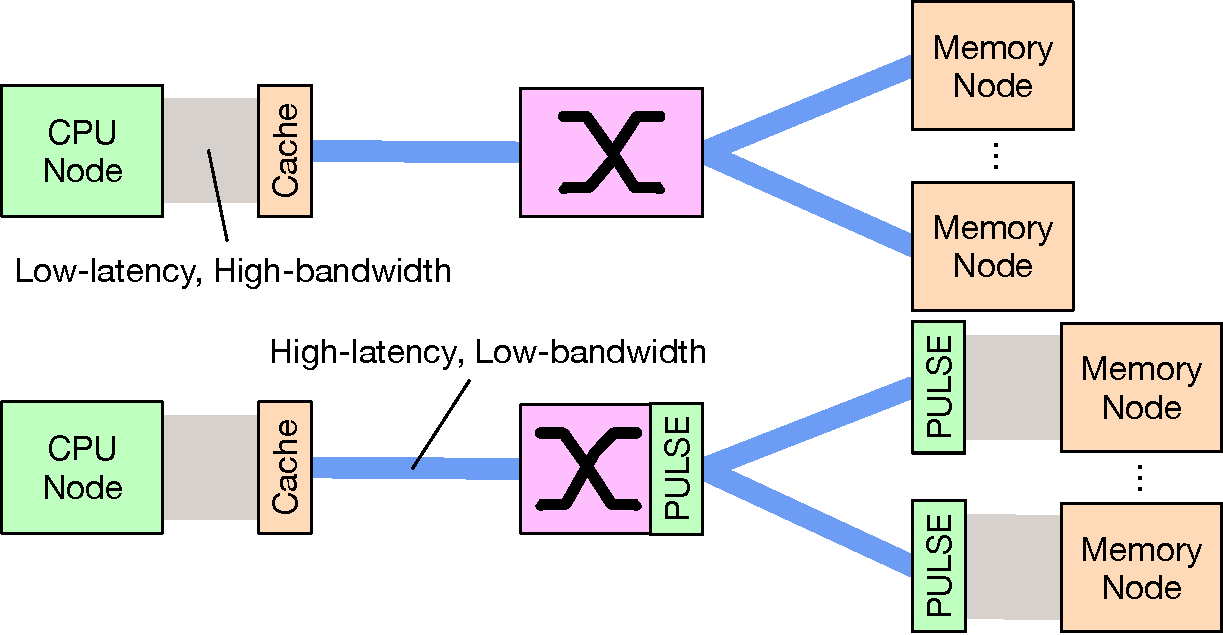
\includegraphics[width=0.98\columnwidth]{fig/pulse/disagg_vertical.pdf}
  \vspace{-0.7em}
  \caption{\textbf{Need for accelerating pointer traversals.} \textit{(top)} The performance of pointer traversals in disaggregated architectures is bottlenecked by slow memory interconnect. \textit{(bottom)} Just as caches offer limited but fast caches near CPUs, we argue that memory needs a counterpart for traversal-heavy workloads: a lightweight but fast accelerator for cache-unfriendly pointer traversals.} 
  \label{fig:disagg}%\vspace{-1.5em}
\end{figure}

\begin{figure*}[ht!]
    \centering
    \subfigure[Our empirical analysis]{
        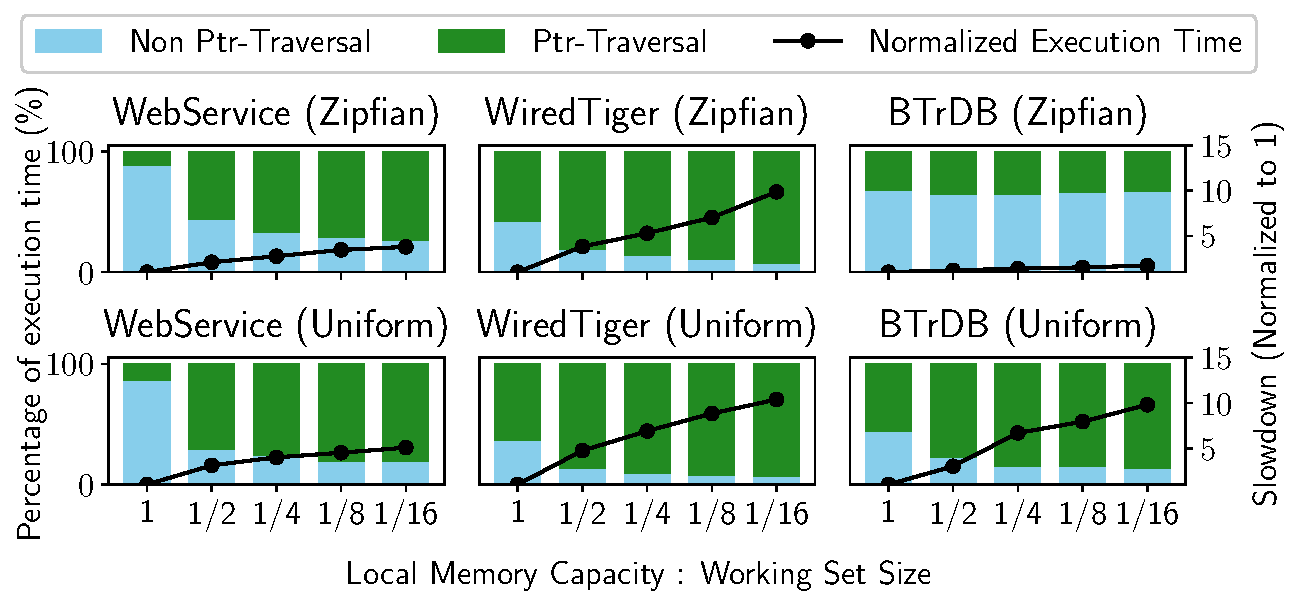
\includegraphics[width=0.49\textwidth]{figure1_motivation.pdf}
        \label{fig:motivation_experiment}
    }
    \subfigure[\% of distributed traversals]{
        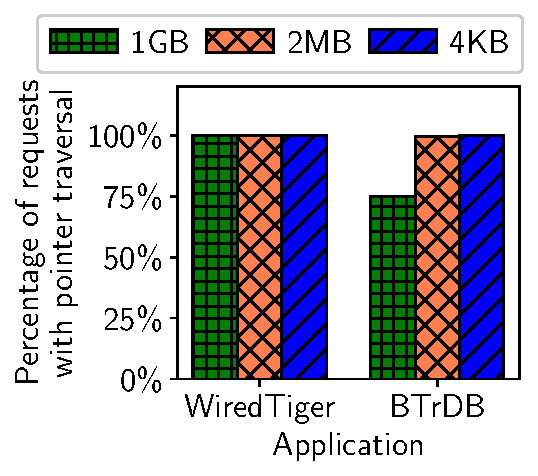
\includegraphics[width=0.21\textwidth]{distributed.pdf}
        %\vspace{1pt}
        \label{fig:distributed_percentage}
    }
    \subfigure[CDF of distributed traversals]{
        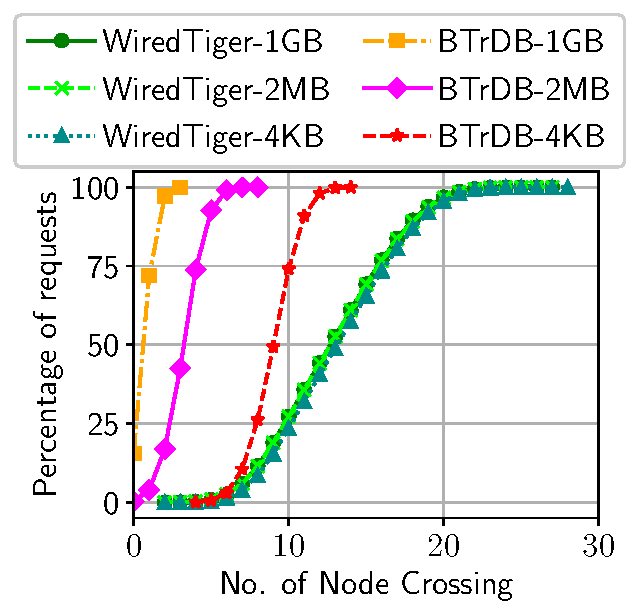
\includegraphics[width=0.24\textwidth]{cdf.pdf}
        \label{fig:distributed_cdf_wiredtiger}
    }
    \vspace{-1em}
    \caption{\textbf{Time cloud applications spend in pointer traversals.} See \S\ref{ssec:need} for details.} %(a) A survey of prior studies~\cite{impica, walkers, charon, xmem}. 
   %(a) Our own empirical analysis shows that pointer traversals constitute a large fraction of the overall application execution time ($13.6\%$--$63.7\%$), with the fraction increasing (along with end-to-end execution time) as less of the application data is cached close to the compute node (or more of the data is remote).  (b) Even with large 1 GB allocations, $>97$\% and $75$\% of requests require cross-node pointer traversals. (c) Since B+Tree nodes are spread across memory nodes due to random data insertion order in WiredTiger, cross-node traversals remain high for all allocation granularities. Time-ordered data insertion in BTrDB permits larger allocation granularities to reduce the number of cross-node traversals, albeit smaller allocation granularities require more.}
    \label{fig:motivation}%\vspace{-1.5em}
\end{figure*}

% Prescriptive and requirements
% Just as caches provide small amounts of fast memory close to the CPU for faster access to popular data, we believe memory nodes should have lightweight processing units to accelerate pointer-traversal workloads with poor cache locality. 
Similar to how CPUs have small but fast memory (\ie, caches) for quick access to popular data, we argue that memory nodes should also include lightweight but fast processing units with high-bandwidth, low-latency access to memory to speed up pointer-traversals (Fig.~\ref{fig:disagg}~(bottom)). Moreover, the interconnect should facilitate efficient and scalable distributed traversals for deployments with multiple memory nodes that cater to large-scale linked data structures. Prior works have explored systems and API designs for such processing units under multiple settings, ranging from near-memory processing and processing-in-memory approaches~\cite{ahn2015scalable, asghari2016chameleon,  dai2018graphh, schuiki2018scalable, mutlu2019processing, lockerman2020livia, tu2022redcim, devic2022_PIM, wang2022_Nearstream, xie2023mpu, mutlu2022modern, oliveira2022accelerating, eckert2022eidetic, chi2016prime, seshadri2017simple, kwon2019_TensorDIMM, boroumand2019_codna, cho2020_data, ke2020_RecNMP, wang2021stream, xie2021spacea, ke2021near, singh2021fpga, olgun2022pidram, dai2022dimmining, gu2020ipim, gomez2023evaluating, walkers, impica} for single-server architectures, to the use of CPUs~\cite{storagefunctions, splinter, aifm, kayak_nsdi_21, storm_systor_19, zhang2022_teleport} or FPGAs~\cite{clio, strom} near remote/disaggregated memory, but have several key shortcomings. 
% \abhishek{Look up Onur Mutlu, Yuan Xie, Daniel Sanchez, Nathan Bechmann, Reetu Das, etc, and cite their papers; take a look at which papers have cited theirs and identify more near-memory processing papers. You will want architects to concede that you know the related work from the architecture community.}
%\slee{} \slee{I will just leave empty comment to mark the location I modified}

% Related work
Specifically, existing approaches are limited in scale and expose a three-way tradeoff between expressiveness, energy efficiency, and performance. First, and perhaps most crucially, none of the existing approaches can accelerate pointer traversals that span \emph{multiple} network-attached memory nodes. 
%\abhishek{This needs to be defined carefully---does this also include memory attached to sockets that are part of the same addressable physical address space? Or is this specifically pertaining to memory nodes that are separated by a packet-switched network rather than an on-chip network?} \anurag{Tried to clarify this.} 
This limits memory utilization and elasticity since applications must confine their data to a single memory node to accelerate pointer traversals. Their inability to support distributed pointer traversals stems from complex management of address translation state that is required to identify if a traversal can occur locally or must be re-routed to a different memory node (\S\ref{ssec:prior}). Second, existing single-node approaches use full-fledged CPUs for expressive and performant execution of pointer-traversals~\cite{storagefunctions, splinter, aifm, kayak_nsdi_21}. However, coupling large amounts of processing capacity with memory --- which has utility in reducing data movement in PIM architectures~\cite{ahn2015scalable, dai2018graphh, schuiki2018scalable, mutlu2019processing, mutlu2022modern, oliveira2022accelerating, eckert2022eidetic, xie2023mpu, tu2022redcim, lockerman2020livia, asghari2016chameleon, devic2022_PIM, wang2022_Nearstream} ---  goes against the very spirit of memory disaggregation since it leads to poor utilization of compute resources and, consequently, poor energy efficiency. 
%\abhishek{The last sentence should be worded a bit carefully; all this processing capacity seems unnecessary to *us* because we're only considering graph processing by design---I would reword to say that those prior studies don't capture how efficient you could get if you only considered graph traversal, which is such a domain of importance/inefficiency in near-memory processing that it is worth considering even on its own.} \anurag{I see your point, but I do want to emphasize that attaching a full-fledged CPU to a memory node does defeat the purpose of disaggregation. At the time of writing, that seemed like a stronger argument than saying it is possible to design more efficient accelerators (which is more of our solution rather than a problem with prior approaches).} 
Approaches that use wimpy processors at SmartNICs~\cite{rmc_hotnets20, redn} instead of CPUs retain expressiveness, but the limited processing speeds of wimpy nodes curtail their performance and, ultimately lead to lower energy efficiency due to their lengthened executions (\S\ref{ssec:application-study},~\cite{clio}). Lastly, FPGA-based~\cite{clio, strom, sun2023demystifying} and ASIC-based~\cite{impica, walkers} approaches achieve performance and energy efficiency by hard-wiring pointer traversal logic for specific data structures, limiting their expressiveness.  %Moreover, the tradeoffs made by all prior approaches worsen significantly when applied to distributed pointer traversals.
% \abhishek{I think precisely defining what a memory node means would help here.}\slee{Agreed; for instance, starting from Fig. 1, we can use `memory server' instead of memory node, and/or draw physical boundary of the server.} \abhishek{I don't get this---are you saying that lower performance means longer-running workloads and so static energy adds up, leading to overall energy inefficiency?} \anurag{Pretty much, yes; but didn't want to spend too much real-estate on this. What would be a more clear/succinct way of saying this?}

% \slee{I relocated a part of this to the earlier paragraph. I think the remaining discussion of Intel's FGPA and general CXL technology should be merged into related work (or just skipped).}
% \yupengnew{\sout{Recently, the industry has embraced Compute Express Link(CXL) as a high-performance interconnect for memory disaggregation. While \name was not originally built on CXL due to the unavailability of CXL hardware at that time, we believe that \name can provide advantages to any disaggregated memory system, regardless of the interconnect technology. \name can bridge the latency gap between faster memory near the CPU (e.g., 10-20 ns of L3 cache) and slower memory far from the CPU (e.g., ~300 ns of CXL memory~\cite{pond}). Intel's recent work~\cite{sun2023demystifying} also envisioned FPGA-based CXL devices, taking advantage of the programmability of FPGA for enabling custom processing}}

We design \name\footnote{\textbf{P}rocessing \textbf{U}nit for \textbf{L}inked \textbf{S}tructur\textbf{E}s.}, a distributed pointer-traversal framework for rack-scale disaggregated memory, to meet all of the above needs --- namely, expressiveness, energy efficiency, performance --- via a principled redesign of near-memory processing for disaggregated memory. Central to \name's design is an expressive iterator interface that readily lends itself to a unifying abstraction across most pointer traversals in linked data structures used in key-value stores~\cite{redis, memcached}, databases~\cite{wiredtiger, btree1, btree2, trie1, trie3}, and big-data analytics~\cite{powergraph, graphx, graphchi, pagerank} (\S\ref{sec:interface}). \name's use of this abstraction not only makes it immediately useful in this large family of real-world traversal-heavy use cases, but also enables (i) the use of familiar compiler toolchains to support these use cases with little to no application modifications and (ii) the design of tractable hardware accelerators and efficient distributed traversal mechanisms that exploit properties unique to iterator abstractions.

%Indeed, our iterator interface can realize most of the linked data structure operations. \abhishek{This is nice---I think that you can say something stronger here about why the iterator is a really clean abstraction to place in the hardware/software contract because it's familiar to programmers, enables them the flexibility to support many graphs, and can be supported efficiently by the underlying hardware (something that you will show).} \anurag{Could use your help in saying this more clearly!}

In particular, \name enables transparent and efficient execution of pointer traversals for our iterator abstraction via a novel accelerator that employs a \emph{disaggregated} architecture to decouple logic and memory pipelines, exploiting the inherently sequential nature of compute and memory accesses in iterator execution (\S\ref{sec:accelerator}). This permits high utilization by provisioning more memory and fewer logic pipelines to cater to memory-centric pointer traversal workloads. A scheduler breaks pointer traversal logic from multiple concurrent workloads across the two sets of pipelines and employs a novel multiplexing strategy to maximize their utilization. While our implementation leverages an FPGA-based SmartNIC due to the high cost and complexity of ASIC fabrication, our ultimate vision is an ASIC-based realization for improved performance and energy efficiency. 
% \abhishek{I think that this first sentence doesn't capture the main point---I think you're saying that you will show how to build a novel accelerator that decouples logic and pipelines and then show the path to it with an FPGA prototype as a precursor to ASIC implementation. Basically, have the first sentence convey the central insight, which is to emphasize what is novel about this accelerator.}\slee{Yes, for ASPLOS submission, I think we should emphasize the accelerator design and its novelty first before showing our effort to build an FPGA-based prototype.}
%Our accelerator  %Finally, an offload engine at the CPU node performs static analysis to ensure traversals are offloaded to the accelerator only if it improves application performance. % on an FPGA-based SmartNIC

We enable distributed traversals by leveraging the insight that pointer traversal across network-attached memory nodes is equivalent to packet routing at the network switch (\S\ref{sec:distributed}). As such, \name leverages a programmable network switch to inspect the next pointer to be traversed within iterator requests and determine the next memory node to which the request should be forwarded --- both at line rate. % to facilitate distributed pointer traversals . \abhishek{Again, the contribution is the insight---the implementation of doing this over a programmable network switch is a consequence of that insight as a prototype. Reverse the order in which this is presented.} This builds on our observation that pointer traversal across disaggregated memory nodes is equivalent to packet routing at the network switch. As such, the programmable switch

We implement a real-system prototype of \name on a disaggregated rack of commodity servers, SmartNICs, and a programmable switch with full-system effects. None of \name's hardware or software changes are invasive or overly complex, ensuring deployability.  Our evaluation of end-to-end real-world workloads shows that \name outperforms disaggregated caching systems with $9$--$34\times$ lower latency and $28$--$171\times$ higher throughput. Moreover, our Xilinx XRT~\cite{xilinx_xrt} and Intel RAPL~\cite{intel_rapl}-based power analysis shows that \name consumes $4.5$--$5\times$ less energy than RPC-based schemes (\S\ref{sec:evaluation}). % \abhishek{Use the word real system with full-system effects with end-to-end workload analysis here to convey that the evaluation is superior to most ASPLOS papers, which use simulated performance models, eschew full system effects, and run tiny instruction snippets from workloads.} \abhishek{If you use circuit-level tools to estimate power numbers post-physical synthesis, say that because that will be more fidelity than most ASPLOS papers.}


